
\documentclass[border=1pt]{standalone}
\usepackage[T1]{fontenc}
\usepackage{newtxtext}
\usepackage{newtxmath}
\usepackage{amsmath}
\usepackage{tikz}
\usepackage{pgfplots}
\usepgfplotslibrary{groupplots}
\usetikzlibrary{arrows.meta}
\pgfplotsset{compat=1.18}

\definecolor{cclassical}{HTML}{2166ac}
\definecolor{clearned}{HTML}{b2182b}
\definecolor{cproposed}{HTML}{1a9850}
\definecolor{cref}{HTML}{7f7f7f}
\definecolor{clight}{HTML}{67a9cf}
\definecolor{cbandlo}{HTML}{f4a582}
\definecolor{cbandhi}{HTML}{92c5de}

% Figure text is sized for a 252 pt column: axis labels a touch under the
% 8 pt caption size, tick labels one step below that.
\newcommand{\figlab}{\fontsize{7.5}{8.5}\selectfont}
\newcommand{\figtick}{\fontsize{6.5}{7.5}\selectfont}
\newcommand{\fignote}{\fontsize{6}{7}\selectfont}

\pgfplotsset{
  every axis/.append style={
    line width=0.5pt,
    scale only axis,
    tick style={line width=0.4pt, black},
    tick pos=left,
    grid=major,
    grid style={gray!30, line width=0.3pt},
    label style={font=\figlab},
    tick label style={font=\figtick},
    title style={font=\figlab, yshift=-2pt},
    legend cell align=left,
    legend style={
      font=\fignote, draw=black!35, fill=white, fill opacity=0.92,
      text opacity=1, inner sep=1.2pt, row sep=-1.5pt, legend image post style={scale=0.7}},
  },
  every axis plot/.append style={line width=0.7pt, mark size=1.3pt},
}
\begin{document}
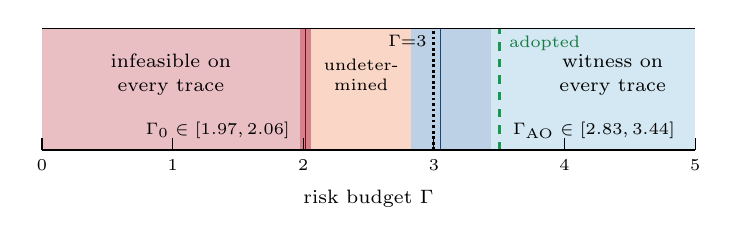
\begin{tikzpicture}
\begin{axis}[
  width=236pt, height=44pt,
  xmin=0, xmax=5, ymin=0, ymax=1,
  ytick=\empty, axis y line=none, xlabel={risk budget $\Gamma$},
  xtick={0,1,2,3,4,5}, grid=none, axis on top]
\fill[clearned, opacity=0.28] (axis cs:0,0) rectangle (axis cs:1.97372,1);
\fill[cbandlo, opacity=0.45] (axis cs:2.06071,0) rectangle (axis cs:2.82625,1);
\fill[cbandhi, opacity=0.40] (axis cs:3.43841,0) rectangle (axis cs:5,1);
\fill[clearned, opacity=0.55] (axis cs:1.97372,0) rectangle (axis cs:2.06071,1);
\fill[cclassical, opacity=0.30] (axis cs:2.82625,0) rectangle (axis cs:3.43841,1);
\draw[clearned!60!black, line width=0.6pt] (axis cs:2.01856,0) -- (axis cs:2.01856,1);
\draw[cclassical!70!black, line width=0.6pt] (axis cs:3.05008,0) -- (axis cs:3.05008,1);
\draw[black, densely dotted, line width=1.0pt] (axis cs:3,0) -- (axis cs:3,1);
\draw[cproposed, dashed, line width=1.0pt] (axis cs:3.5,0) -- (axis cs:3.5,1);
\node[font=\figlab, align=center] at (axis cs:0.986858,0.62) {infeasible on\\every trace};
\node[font=\fignote, align=center] at (axis cs:2.44348,0.62) {undeter-\\mined};
\node[font=\figlab, align=center] at (axis cs:4.3692,0.62) {witness on\\every trace};
\node[font=\fignote, anchor=east, inner sep=1pt] at (axis cs:1.92372,0.16) {$\Gamma_0\in[1.97,2.06]$};
\node[font=\fignote, anchor=west, inner sep=1pt] at (axis cs:3.58,0.16) {$\Gamma_{\mathrm{AO}}\in[2.83,3.44]$};
\node[font=\fignote, anchor=north east, inner sep=1pt] at (axis cs:2.97,0.97) {$\Gamma{=}3$};
\node[font=\fignote, anchor=north west, inner sep=1pt, text=cproposed!80!black] at (axis cs:3.55,0.97) {adopted};
\end{axis}
\end{tikzpicture}
\end{document}
